%%%%%%%%%%%%%%%%%%%%%%%%%%%%%%%%%%%%%%%%%%%%%%
\section{Généralités}
%%%%%%%%%%%%%%%%%%%%%%%%%%%%%%%%%%%%%%%%%%%%%%

 \begin{frame}{Naissance de logiciel libre}{}
  \begin{itemize}
  \item 1983: Richard Stallman - Projet \textbf{GNU} et concept de logiciel libre. Developpement de gcc, gdb, glibc, etc
  \item 1991: Linus Torvalds - Projet noyau (\textbf{kernel}) \textbf{Linux}. De type Unix
  \item 1995: Linux est de plus en plus populaire sur les serveurs
  \item 2000: Linux est de plus en plus populaire sur les \textbf{systèmes embarqués}
  \item 2008: Linux est de plus en plus populaire sur les appareils mobiles
  \item 2010: Linux est de plus en plus populaire sur les téléphones
  \end{itemize}
\end{frame}

\begin{frame}{Logiciel libre ?}{}
  \begin{itemize}
  \item Un logiciel est considéré libre quand sa license respecte ces \textbf{4 libertés}:
    \begin{itemize}
    \item Liberté d'\textbf{éxécuter} le logiciel pour n'importe quel but
    \item Liberté d'\textbf{étudier} le logiciel et de le \textbf{modifier}
    \item Liberté de \textbf{redistribuer} des copies
    \item Liberté de \textbf{distribuer} des copies modifiées
    \end{itemize}
  \item Le code doit être disponible, le logiciel peut être modifié et distribué aux utilisateurs
  \end{itemize}
  \center\textbf{Parfait pour les systèmes embarqués !}
\end{frame}

\begin{frame}{Historique de Linux}{}
  \begin{itemize}
  \item Créé par Linus Torvalds en 1991
  \item Est un noyau : logiciel gérant les ressources d'une machine
  \item N'est pas un système d'exploitation : est lié au projet GNU\\
    \MVRightarrow{} distribution GNU/Linux
  \end{itemize}
\end{frame}

\begin{frame}{Linux dans l'industrie}{}
  L'intérét pour les entreprise est:
  \begin{itemize}
  \item de maitriser les sources de leur OS
  \item d'économiser le prix des licences
  \item de bénéficier du support d'une communauté importante de développeur
  \item d'utiliser des composants déjà existants et testés par X personnes
  \end{itemize}
  Seule la partie Desktop a du mal face à ses concurrents
 \end{frame}

\subsection{Concepts}

\begin{frame}{Basé sur UNIX}{}
  \begin{itemize}
  \item Implémentation libre d'UNIX diffusé sous licence GPL
  \item Inspiré des deux versions: AT\&T et BSD
  \item Les principes d'UNIX sont respectés:
  \begin{itemize}
  \item Simplicité, modularité, respect des standards, ouverture
  \item Abstraction du système : noyau = matériel ; userspace = applications
  \item Le noyau permet d'accéder au matériel (pilotes, appels système)
  \item Tout composant est un \textbf{fichier}: répertoire, périphérique, élément de communication, etc. (organisation arborescente)
  \item Puissance de la "ligne de commande" (shell et regexpr)
  \end{itemize}
  \end{itemize}
\end{frame}

\begin{frame}{Architecture}{}
  \begin{center}
    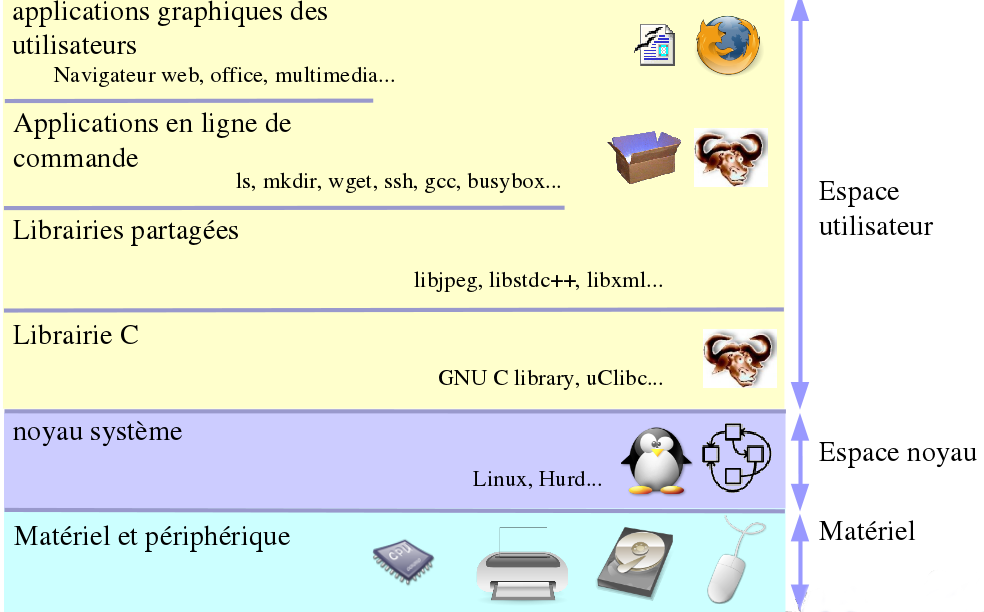
\includegraphics[height=0.8\textheight]{pictures/architecture-unix.png}
  \end{center}
\end{frame}

\begin{frame}{Fonctionnalitées}{}
  \begin{itemize}
  \item Noyau monolithique (en un seul fichier) + modules dynamiques
  \item Création des processus via fork() et exec()
  \item Multi-threading
  \item Nombreuses piles réseau (IPv4, IPv6, Ethernet, etc.)
  \item Organisation des fichiers arborescente à partir de la racine (/), montage et démontage logique (mount)
  \item Multi-utilisateurs avec un super-utilisateur (root) et des groupes
  \end{itemize}
\end{frame}

\subsection{Licence}

\begin{frame}{GPL en bref}{}
  \begin{itemize}
  \item GPL General Public License
  \item On la surnomme également copyleft
  \item La GPL v2 (1991) est la plus répandue (ex: noyau Linux)
  \item La licence s'applique uniquement en cas de redistribution
  \item Un code source utilisant du code GPL est du travail dérivé et doit être publié
  \item Publication: celui qui reçoit la version binaire peut obtenir le code source
  \item Pas de lien (ld) possible entre du code GPL et du code propriétaire
  \end{itemize}
\end{frame}

\begin{frame}{LGPL}{}
  \begin{itemize}
  \item La GPL est complexe à gérer dans l'industrie \MVRightarrow{} création de la LGPL
  \item Le lien avec du code propriétaire est possible avec la LGPL (Lesser/Library GPL) !
  \item En majeure partie, les bibliothèques système sont diffusées sous LGPL (exemple: GNU-libc)
  \item Dans le cas d'une application propriétaire il faut donc vérifier qu'aucune bibliothèque liée n'est GPL
  \item Le lien dynamique n'affranchit pas de la licence sauf dans des cas très particuliers
  \end{itemize}
\end{frame}

\begin{frame}{GPL uniquement pour LINUX}{}
  \begin{itemize}
  \item Dans l'espace noyau (pilotes), SEULE la GPL s'applique (en théorie) !
  \item En théorie: On ne peut utiliser les headers du noyau Linux pour créer des binaires non GPL
  \item Certaines fonctions ne sont pas disponibles si la licence n'est pas GPL
  \item En pratique: tolérance si le pilote n'a pas été créé pour Linux (cas du portage) \MVRightarrow{} nVidia, Broadcom, ...
  \item Cependant les pilotes binaires posent des soucis techniques vu qu'un pilote fonctionne pour la version de noyau utilisée pour la compilation
  \end{itemize}
\end{frame}

\begin{frame}{GPL V3}{}
  \begin{itemize}
  \item Nouvelle version sortie en 2007
  \item Oblige à fournir les éléments pour construire un logiciel fonctionnel \MVRightarrow{} réponse à la Tivoisation
  \item La GPL v2 demande uniquement la publication des sources à celui qui a reçu le binaire
  \item La GPL v3 ne sera pas utilisée pour le noyau Linux
  \item Voir: http://www.gnu.org/licenses/quick-guide-gplv3.fr.html
  \end{itemize}
\end{frame}

%%%%%%%%%%%%%%%%%%%%%%%%%%%%%%%%%%%%%%%%%%%%%%
\section{Architecture GNU/Linux}
%%%%%%%%%%%%%%%%%%%%%%%%%%%%%%%%%%%%%%%%%%%%%%

\begin{frame}{Système GNU/Linux}{}
  \begin{itemize}
  \item Noyau libre semblable à un noyau Unix, conçu par Linus Torvalds en 1991
  \item Le système complet se repose sur les outils GNU:
    \begin{itemize}
    \item bibliothèque C, gcc, binutils, fileutils, make, emacs...
    \item Le système complet est donc appelé "\textbf{GNU / Linux}"
    \end{itemize}
  \item Très tôt partagé comme Logiciel Libre (Licence GPL) \MVRightarrow attira des contributeurs et des utilisateurs de plus en plus nombreux
  \item Maintenant, fournit en tant que "distribution" (Ubuntu, Fedora, Debian, etc)
  \item Système entier composé de:
    \begin{itemize}
    \item Un bootloader (Rares sont les cartes capable de booter un noyau Linux)\\
      Il est trop gros et doit etre chargé en RAM. Elle doit etre initialisée par un microcode avant \MVRightarrow{} Utilité du \textbf{bootloader}
    \item Le noyau Linux qui gére les ressources de la machine
    \item Un système de fichier contenant à minima un programme de démarrage (rootfs)
    \end{itemize}
  \end{itemize}
\end{frame}

\begin{frame}{Noyau}{}
  \begin{itemize}
  \item Le noyau Linux est un binaire de type ELF
  \item Son image est souvent compressée pour gagner en taille lors du déploiement et de la copie en RAM
  \item Il contient un auto extracteur qui va le décomprésser
  \item Fournit des services nécéssaires à sa fonction:
    \begin{itemize}
    \item ordonanceur
    \item gestion mémoire, disque, interface réseaux
    \item service abtraits (systeme de fichier, pile réseaux ...)
    \end{itemize}
  \item Une grande partie du noyau peut etre déporté en \textbf{module} chargé dynamiquement
  \end{itemize}
\end{frame}

\begin{frame}{Architecture}{Noyau}
  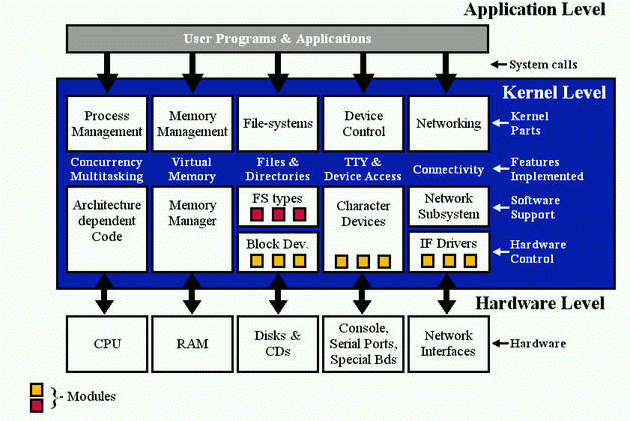
\includegraphics[width=10cm]{pictures/kernel_arch.png}
\end{frame}

\begin{frame}{Module noyau}
  \begin{itemize}
  \item Modules noyau: .ko (Kernel Object)
  \item Les modules binaires sont liés à la version du noyau !
  \item Peut se compiler après mais nécessite les entetes du noyau
  \item Mécanisme système pour charger les modules dynamiquement: modprobe, insmod, rmmod
  \end{itemize}
\end{frame}

\begin{frame}{Organisation d'un rootfs}
  \begin{itemize}
  \item Organisation commune à 90\% entre les UNIX
  \item Quelques spécificités GNU/Linux et distribution
  \item Tout commence depuis la racine \texttt{/}
  \item Puis, organisation en dossier/sous-dossier:
    \begin{itemize}
    \item \texttt{/bin,/sbin,/usr/bin,/usr/sbin}: binaires communs et systèmes
    \item \texttt{/lib,/usr/lib}: bibliothèques et modules noyau
    \item \texttt{/etc}: fichiers de configuration
    \item \texttt{/dev}: nœuds d'accès aux périphériques
    \item \texttt{/var}: fichiers variables comme log, mail, ...
    \item \texttt{/opt}: pour les programmes externes (ex: LibreOffice)
    \item \texttt{/home}: accueille les répertoires des utilisateurs
    \end{itemize}
  \end{itemize}
\end{frame}

\begin{frame}{Organisation d'un rootfs}
  \begin{itemize}
  \item Quelques répertoires spéciaux:
    \begin{itemize}
    \item \texttt{/lib/modules}: contient les modules du noyau
    \item \texttt{/root}: home-directory de l'utilisateur root
    \item \texttt{/media}: point de montage des volumes amovibles
    \item \texttt{/proc}: système de fichier virtuel (état du système)
    \item \texttt{/sys}: idem pour les périphériques connectés
    \item \texttt{/boot}: noyau statique (vmlinuz, uImage, ...)
    \end{itemize}
  \end{itemize}
\end{frame}

\begin{frame}{/proc}
  \begin{itemize}
  \item Système de fichier virtuel (lecture/écriture) géré par le noyau. (Réponse sur solicitation, pas d'écriture sur un support)
  \item Intérêt: manipuler les variables systèmes comme de fichiers (cat, echo, grep)
  \item Exemples:
    \begin{itemize}
    \item \texttt{/proc/version}: version du noyau
    \item \texttt{/proc/cpuinfo}: type(s) de processeur(s)
    \item \texttt{/proc/interrupts}: interruptions
    \item \texttt{/proc/pid}: répertoire décrivant le processus associé au pid
    \item \texttt{/proc/mounts}: partitions montées
    \item \texttt{/proc/modules}: liste des modules noyau chargés
    \end{itemize}
  \item Nombreuses commandes systèmes basées sur \texttt{/proc} : lsmod, lspci, top, mount, ...
  \end{itemize}
\end{frame}

\begin{frame}{/sys}
  \begin{itemize}
  \item Introduit dans le noyau 2.6 (2003) \MVRightarrow{} sysfs
  \item Vue synthétique des périphériques connectés
    \begin{itemize}
    \item \texttt{/sys/class}
    \item \texttt{/sys/modules}
    \item \texttt{/sys/bus}
    \end{itemize}
  \item But: mieux gérer l'ajout/suppression dynamique des périphériques (hotplug)
  \item Utilisé par UDEV pour créer dynamiquement les entrées dans \texttt{/dev}
  \item Quelques recouvrements avec /proc (bus PCI, USB, ...)
  \end{itemize}
\end{frame}

\section{Execution d'un système GNU/Linux}

\begin{frame}{Démarrage}
  \begin{columns}
    \column{0.6\textwidth}
    \begin{enumerate}
    \item Le matériel lance le bootloader
    \item Le bootloader configure la RAM et le support contenant le noyau
    \item Le bootloader copie le noyau en RAM et lui donne la main
    \item Le noyau s'auto extrait en RAM
    \item Le noyau initialise les périphériques et les sub-systèmes (ordonnanceur, pile réseaux, sytème de fichier,...)
    \item Le noyau récupère dans le rootfs le binaire d'initialisation (\texttt{/sbin/init} par défaut) et crée le processus 1
    \item Ce processus est chargé de démarrer tous les services en espaces utilisateurs
    \end{enumerate}
    \column{0.4\textwidth}
    \begin{center}
      \includegraphics[height=0.7\textheight]{graphics/overall-boot-sequence.pdf}
    \end{center}
  \end{columns}
\end{frame}

\begin{frame}{Le processus init}
  \begin{itemize}
  \item Le père des processus du système
  \item Plusieurs systèmes possible:
    \begin{itemize}
    \item system5:
      \begin{itemize}
      \item facile à configurer car basé sur des scripts shell
      \item architecture vieille et dépassé. Moins performant
      \end{itemize}
    \item systemd:
      \begin{itemize}
      \item Parallélise l'initialisation du système. Centralise de nombreux services (logs, etc)
      \item Plus complexe à prendre en main et moins modulaire pour certain
      \end{itemize}
    \item custom:
      \begin{itemize}
      \item Linux permet d'utiliser son propre binaire init.
      \item Il faut gérer soit même le système.
      \end{itemize}
    \end{itemize}
  \end{itemize}
\end{frame}
